%!TEX root = ../../Master.tex
\subsection{Formål}

Formålet med dette projekt er at udvikle et robotsystem.
Der er fra kursets undervisere stillet krav om at systemet skal benytte sig af robotten AX-12A Smart Robotic Arm fra firmaet CrustCrawler Robotics.
Desuden er der stillet et krav om at systemet skal indeholde et vision system. \\

Det er valgt at udvikle et system til farvesortering af klodser.
Vision systemet skal detektere klodsernes placering og farve.
Herefter skal CrustCrawler robotten bruges til at samle klodserne med samme farve i en gruppe.
Grupperne skal være tydeligt adskilt.
Systemet skal blot kunne håndtere to forskellige farver. \\

\fixme{Ændre 'Figure' til 'Figur'}

\begin{figure}[h]
\centering
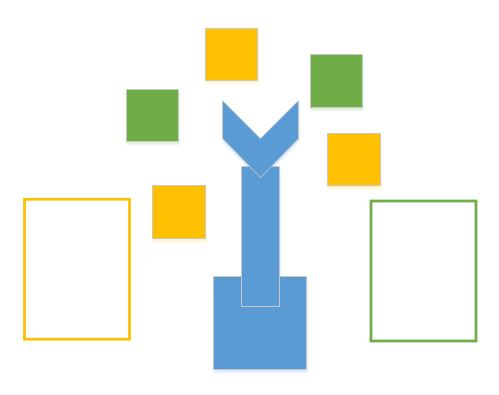
\includegraphics[scale=0.65]{images/purpose}
\caption{Idé til system setup}
\label{fig:purpose}
\end{figure}

En idé til system setup er illustreret på figur \ref{fig:purpose}.
Her ses robotten som den blå figur i midten. De grønne og gule kvadrater er de farvede klodser, som systemet skal kunne sortere. 
De farvede og firkantede omrids i siderne er de steder, hvor klodserne skal grupperes efter farve igennem sorteringen.
Disse markeringer forekommer kun på illustrationen og vil ikke være at finde i det endelige system. \\